\begin{anexosenv}

\partanexos

\chapter{Documento de Visão}

\section{Introdução}

\subsection{Finalidade}

A finalidade deste documento é fornecer uma visão geral da aplicação de aquisição e manipulação dos dados do motor a combustão, apresentando uma visão das macro-funcionalidades do software. Além disso, objetiva-se apresentar as razões pelas quais o sistema será construído.

\subsection{Escopo}

A aplicação destina-se ao suporte ao usuário da bancada, com intuito de fornecer a visualização de informações a cerca do funcionamento do motor no momento da análise de forma gráfica. Tais informações são: Temperatura do óleo do motor; Temperatura do ar no coletor de admissão; Pressão do ar no coletor de admissão; Informações de emissão e mistura sonda/lâmbda.

\section{Posicionamento}

\subsection{Descrição do problema}

\begin{table}[h!]
	\centering
	\caption{Descrição do problema.}
	\label{descricaoproblema}
	\begin{tabular}{|l|l|}
		\hline
		\textbf{O problema de}                                                    & \begin{tabular}[c]{@{}l@{}}Dificuldade de se analisar os parâmetros e características de um,\\ motor em funcionamento.\end{tabular}                                      \\ \hline
		\textbf{Afeta}                                                            & Estudantes e professores do curso de engenharia automotiva.                                                                                                              \\ \hline
		\textbf{Cujo impacto é}                                                   & \begin{tabular}[c]{@{}l@{}}Impossibilidade, por parte dos alunos, de conhecer e analisar\\ parâmetros e características de um motor a combustão na prática.\end{tabular} \\ \hline
		\textbf{\begin{tabular}[c]{@{}l@{}}Uma boa solução \\ seria\end{tabular}} & \begin{tabular}[c]{@{}l@{}}Utilizar recursos gráficos, por meio de um software, para dar \\ suporte na análise dos dados de um motor em funcionamento.\end{tabular}      \\ \hline
	\end{tabular}
\end{table}

\newpage

\subsection{Sentença de posição do produto}

\begin{table}[h!]
	\centering
	\caption{Sentença de posição do produto}
	\label{my-label}
	\begin{tabular}{|l|l|}
		\hline
		\textbf{Para}            & Compor a bancada de análise                                                                                                                                                              \\ \hline
		\textbf{Que}             & \begin{tabular}[c]{@{}l@{}}Necessita de um sistema de software para dar suporte na visualização\\ das informações do motor.\end{tabular}                                                 \\ \hline
		\textbf{O}               & Software de Aquisição e Processamento de Dados de Motor                                                                                                                                  \\ \hline
		\textbf{Que}             & Auxiliará o usuário da bancada a visualizar as informações do motor                                                                                                                      \\ \hline
		\textbf{Ao contrário de} & Realizar as análises com o veículo completo                                                                                                                                              \\ \hline
		\textbf{A aplicação}     & \begin{tabular}[c]{@{}l@{}}Promoverá uma interface gráfica entre o usuário da bancada e o motor \\ ao qual apresentará as informações referentes ao motor em funcionamento.\end{tabular} \\ \hline
	\end{tabular}
\end{table}


\section{Decrição dos Envolvidos e dos Usuários}

\subsection{Resumo dos envolvidos}

Informações dos stakeholders do projeto de desenvolvimento do software.

\begin{table}[h!]
	\centering
	\caption{Descrição dos envolvidos e dos usuários.}
	\label{descricaoDosEnvolvidos}
	\begin{tabular}{|l|l|l|}
		\hline
		\textbf{Nome}                                                                     & \textbf{Descrição}                                                                                                                                                                              & \textbf{Responsabilidades}                                                                                                                               \\ \hline
		\begin{tabular}[c]{@{}l@{}}Desenvolvedores do \\ software de análise\end{tabular} & \begin{tabular}[c]{@{}l@{}}Alunos de graduação do\\  curso de Engenharia de\\  Software\end{tabular}                                                                                            & \begin{tabular}[c]{@{}l@{}}Análise dos requisitos do \\ software, modelar \\ arquitetura do software,\\ implementar e implantar\\ software.\end{tabular} \\ \hline
		Professores                                                                       & \begin{tabular}[c]{@{}l@{}}Professores da disciplina de \\ Projeto Integrador 2\end{tabular}                                                                                                    & \begin{tabular}[c]{@{}l@{}}Acompanhar e avaliar o \\ desenvolvimento do projeto\end{tabular}                                                             \\ \hline
		\begin{tabular}[c]{@{}l@{}}Equipe de desenvolvimento \\ da bancada\end{tabular}   & \begin{tabular}[c]{@{}l@{}}Alunos de graduação do\\ curso de Engenharia de \\ Energia, Eletrônica, \\ Automotiva, Aeroespacial \\ que compõem a equipe\\ desenvolvedora da bancada\end{tabular} & \begin{tabular}[c]{@{}l@{}}Atuar como clientes,\\ apresentando os problemas\\ que tem que ser resolvidos\\  através da aplicação.\end{tabular}           \\ \hline
	\end{tabular}
\end{table}

\newpage

\subsection{Resumo dos usuários}

Informações dos usuários finais do software.

\begin{table}[h!]
	\centering
	\caption{Usuários finais}
	\label{usuariosfinais}
	\begin{tabular}{|l|l|l|}
		\hline
		\textbf{Nome} & \textbf{Descrição}                                                                       & \textbf{Responsabilidades}                                                                                                                \\ \hline
		Professores   & \begin{tabular}[c]{@{}l@{}}Professores do curso de \\ Engenharia Automotiva\end{tabular} & \begin{tabular}[c]{@{}l@{}}Realizar o acompanhamento \\ geral das informações \\ apresentadas do motor e\\ gerar relatórios.\end{tabular} \\ \hline
		Alunos        & \begin{tabular}[c]{@{}l@{}}Alunos do curso de \\ Engenharia Automotiva\end{tabular}      & \begin{tabular}[c]{@{}l@{}}Realizar o acompanhamento\\ geral das informações \\ apresentadas do motor \\ e gerar relatórios.\end{tabular} \\ \hline
	\end{tabular}
\end{table}

\subsection{Ambiente do usuário}

O software será utilizado diretamente na bancada, pois trata-se de uma aplicação Web executando localmente desenvolvido em Python juntamente com o Framework Django que realizará comunicação com a RaspBerry Pi.

\subsection{Principais necessidades dos usuários ou dos envolvidos}

\begin{table}[h!]
	\centering
	\caption{Necessidades dos usuários ou dos envolvidos}
	\label{necessidadesDosUsuariosOuDosEnvolvidos}
	\begin{tabular}{|l|l|l|}
		\hline
		\textbf{Necessidade}                                                                                                                        & \textbf{Solução atual} & \textbf{Solução proposta}                                                                                                                                      \\ \hline
		\begin{tabular}[c]{@{}l@{}}Realizar o \\ acompanhamento geral\\ das informações \\ apresentadas do motor e\\ gerar relatórios.\end{tabular} & Não há.                & \begin{tabular}[c]{@{}l@{}}Exposição dos dados\\ coletados pelos sensores\\ acoplados ao motor, \\ geração de gráficos, \\ geração de relatórios.\end{tabular} \\ \hline
	\end{tabular}
\end{table}

\section{Visão Geral do Produto}

\subsection{Perspectiva do produto}

Espera-se que o software sirva de auxílio à bancada de testes de um motor a combustão, permitindo uma melhor e mais agradável visualização do funcionamento do equipamento, resultando numa maior facilidade no aprendizado a partir dos alunos.

\subsection{Resumo dos recursos}

Os recursos que o sistema deve conter são funcionalidades importantes para resolver o problema e as necessidades do cliente. Este software conta com as seguintes funcionalidades:

\begin{itemize}
	\item Coleta e Armazenamento de dados - Esta funcionalidade permite que o usuário salve os dados coletados na análise.
	\item Visualização dos resultados - Esta funcionalidade permite que o usuário visualize os resultados da análise realizada por meio de gráficos intuitivos.
	\item Geração de relatório - Esta funcionalidade permite que o usuário gere um relatório a partir de uma análise salva no banco de dados.
\end{itemize}

\section{Recursos do Produto}

\begin{itemize}
	\item O sistema deve coletar os dados do motor dinamicamente transmitidos pela MSP430;
	\item O sistema deve realizar o tratamento dos dados para apresentá-los de forma intuitiva ao usuário;
	\item O sistema deve plotar gráficos a partir dos dados captados;
	\item O sistema deve possuir um botão para que o usuário tenha a opção de salvar todos os dados da análise em um banco de dados;
	\item O sistema deve possuir a opção de gerar um relatório.
\end{itemize}

\section{Restrições}

Nesta seção serão apresentados as restrições de design, restrições externas, como requisitos operacionais ou regulamentares e outras dependências.

São restrições do produto:

\begin{itemize}
	\item O software deverá possuir rotinas para a comunicação UART 12C (para o módulo de aquisição) e GPIO (para o módulo de controle) com um microcontrolador MSP430;
	\item A comunicação entre a RaspBerry Pi e a MSP430 deverá ser dinâmica para que o usuário possa acompanhar o andamento da análise;
	\item O software deverá ser, em essência, uma aplicação Web desenvolvida em Python juntamente com o Framework Django;
	\item O software não deverá realizar o controle de partida e aceleração do motor por questões de segurança.
\end{itemize}

\chapter{Documento de Arquitetura}

\section{Introdução}

Este documento apresenta a arquitetura proposta para o software da bancada de testes de motor que fará o tratamento, exposição dos dados coletados na análise de motor a combustão e o controle do motor. A arquitetura é apresentada através de um conjunto de visões que juntas visam cobrir os principais aspectos técnicos relativos ao desenvolvimento e implantação do sistema em questão. O objetivo é capturar e formalizar as principais decisões tomadas com relação à arquitetura do sistema.

\subsection{Finalidade}

Este documento tem como objetivo apresentar uma arquitetura para sistemas que possuem características de aquisição de dados em “tempo real” a partir de uma placa microcontroladora.

\subsection{Escopo}

O escopo deste documento é documentar as partes significativas do ponto de vista da arquitetura, como sua divisão em camadas e pacotes.

\section{Arquitetura da Aplicação}

O  SBTM - Software da Bancada de Testes de Motor será um sistema web que terá dois módulos de aplicação, sendo eles o módulo de aquisição onde terá uma placa microcontroladora MSP430-2 que irá coletar todos os dados do motor dinamicamente durante a análise e enviá-los para a Raspberry Pi utilizando a comunicação UART 12c, assim, haverá um servidor wifi gerado pela RaspBerry e conectado ao computador que transmitirá os dados para que o software possa gerenciá-los e exibi-los de forma intuitiva ao usuário. Também terá o módulo de controle onde serão feitos os controles de partida e aceleração do motor, que serão feitos através de envio de dados para a MSP430-2 utilizando comunicação GPIO.

Adicionalmente, o software terá um banco de dados na RaspBerry onde serão persistidos os resultados da análise do motor. Sendo assim, será possível ao usuário abrir posteriormente uma análise previamente salva no banco de dados.

\subsection{Representação da Arquitetura}

A figura \ref{diagramaArquitetura} representa o Diagrama de componentes do SBTM:

\begin{figure}[h!]
	\centering
	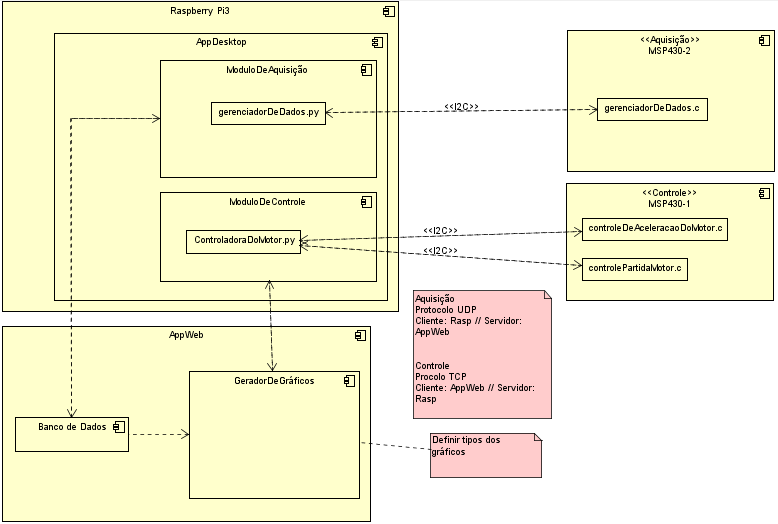
\includegraphics[keepaspectratio=true,scale= 0.7]{figuras/DiagramaDeArquitetura.PNG}
	\caption{Diagrama de Componentes}
	\label{diagramaArquitetura}
\end{figure}

\subsection{Objetivos e Restrições da Arquitetura}

O objetivo dessa arquitetura é modularizar a aplicação de modo a prover um controle no desenvolvimento e facilidade de manutenção do sistema. Além disso, essa arquitetura modularizada provê um ambiente mais propício para implementação de novas features.
A restrição da arquitetura proposta está no poder de processamento da RaspBerry Pi, pois o volume de dados a serem persistidos será relativamente grande o que irá exigir um poder de processamento maior por parte da RaspBerry.

\section{Visão de Casos de Uso}

O SBTM possui inicialmente 8 casos de uso, sendo eles:

\begin{itemize}
	\item UC01 - Realizar acionamento do motor;
	\item UC02 - Realizar a aceleração do motor;
	\item UC03 - Realizar a desaceleração do motor;
	\item UC04 - Salvar informações geradas pela análise do motor;
	\item UC05 - Gerar relatório;
	\item UC06 - Iniciar análise;
	\item UC07 - Apresentar dados do motor dinamicamente;
	\item UC08 - Apresentar gráficos dinâmicos.
\end{itemize}

A figura \ref{diagramaCasoDeUso} apresenta o diagrama de casos de uso do SBTM:

\begin{figure}[h!]
	\centering
	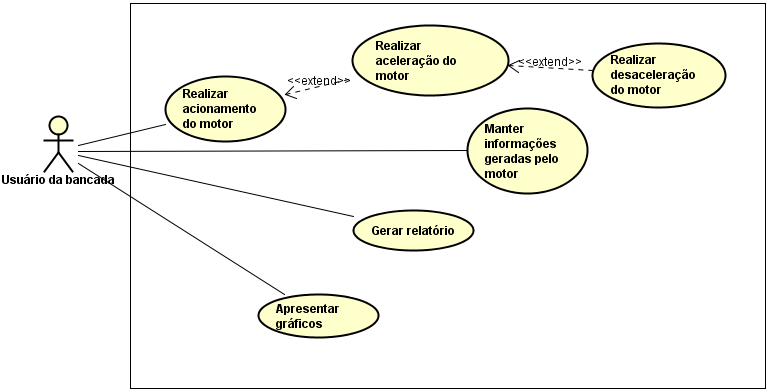
\includegraphics[keepaspectratio=true,scale= 0.7]{figuras/DiagramaDeCasoDeUso.PNG}
	\caption{Diagrama de Caso de Uso}
	\label{diagramaCasoDeUso}
\end{figure}

Observa-se que há uma dependência entre os casos de uso UC01, UC02 e UC03. Esta dependência ocorre pois para que seja possível acelerar o motor (UC02) é necessário que ele seja previamente acionado (UC02), o mesmo ocorre no caso da desaceleração do motor (UC03) pois para que seja possível desacelerar é necessário que o motor esteja acionado e acelerado.

Além disso, observa-se também uma relação de dependência entre os casos de uso UC06, UC07 e UC08. Esta dependência ocorre pois para que o UC07 e UC08 ocorram, é necessário que o UC06 tenha ocorrido, porém o UC07 sempre ocorrerá e o UC08 poderá ocorrer ou não.

\chapter{Terceiro Anexo}

Texto do terceiro anexo.

\end{anexosenv}

